\documentclass[aspectratio=169,11pt]{beamer}
% ==========================================================================
%  KSA lecture-slide theme  =  stock beamer "Boadilla"  +  KSA colour theme
%  brand colours sampled from the official KSA symbol mark:
%    Deep Prussian Blue  #2E3192   (지성 - intellect)
%    Golden Gray         #D6CBB1   (감성 - sensibility)
%  Engine: XeLaTeX.  Usage:
%    \documentclass[aspectratio=169,11pt]{beamer}
%    \input{../../theme/ksa-theme.tex}
%  Each deck lives in its own slides/kor/<deck>/ folder together with its
%  own images; ../../figs/ is kept only as a fallback for the shared cache.
% ==========================================================================

\usepackage{fontspec}
\usepackage{amsmath,amssymb}
\usepackage{graphicx}
\graphicspath{{figs/}{./}{../../../figs/}}
\usepackage{booktabs}
\usepackage{listings}
\usepackage{varwidth}

% ---- fonts (no ctex/xeCJK on this box -> fontspec drives CJK directly) -----
\defaultfontfeatures{Ligatures=TeX}
\setmainfont{Noto Sans CJK KR}
\setsansfont{Noto Sans CJK KR}
\setmonofont{Noto Sans Mono CJK KR}[Scale=0.92]

% ---- base theme: stock Boadilla ------------------------------------------
\usetheme{Boadilla}
\usefonttheme{professionalfonts}
\setbeamertemplate{navigation symbols}{}

% ---- KSA colour theme (recolour the stock theme) --------------------------
\definecolor{ksablue}{HTML}{2E3192}
\definecolor{ksabluedk}{HTML}{20226A}
\definecolor{ksagold}{HTML}{D6CBB1}
\definecolor{ksagolddk}{HTML}{A9976B}
\definecolor{ksared}{HTML}{C0392B}
\definecolor{ksagray}{HTML}{5B5B5B}

\setbeamercolor{structure}{fg=ksablue}
\setbeamercolor{alerted text}{fg=ksared}

\setbeamercolor{palette primary}{fg=white,           bg=ksablue}
\setbeamercolor{palette secondary}{fg=white,         bg=ksablue!85!black}
\setbeamercolor{palette tertiary}{fg=white,          bg=ksabluedk}
\setbeamercolor{titlelike}{fg=ksablue}
\setbeamercolor{frametitle}{fg=ksablue,bg=}
\setbeamercolor{title}{fg=ksablue}
\setbeamercolor{author}{fg=ksagray}
\setbeamercolor{institute}{fg=ksagray}
\setbeamercolor{block title}{fg=white,bg=ksablue}
\setbeamercolor{block body}{fg=black!85,bg=ksablue!6}
\setbeamercolor{item}{fg=ksablue}
\setbeamercolor{section in toc}{fg=black!85}

\setbeamerfont{frametitle}{series=\bfseries}
\setbeamerfont{title}{series=\bfseries}

% ---- footline:  KSA mark | "Made by ..." | n / N   (matches reference) ----
\newcommand{\ksacredit}{}
\setbeamertemplate{footline}{%
  \hbox{%
    \begin{beamercolorbox}[wd=.18\paperwidth,ht=2.6ex,dp=1.5ex,leftskip=1.1em]{}%
      \raisebox{-0.35ex}{\includegraphics[height=2.0ex]{ksa-logo.png}}%
    \end{beamercolorbox}%
    \begin{beamercolorbox}[wd=.64\paperwidth,ht=2.6ex,dp=1.5ex,center]{}%
      {\scriptsize\color{ksagray}\ksacredit}%
    \end{beamercolorbox}%
    \begin{beamercolorbox}[wd=.18\paperwidth,ht=2.6ex,dp=1.5ex,rightskip=1.1em]{}%
      \hfill{\scriptsize\color{ksablue}\insertframenumber\,/\,\inserttotalframenumber}%
    \end{beamercolorbox}%
  }%
  \vskip2pt
}

% ---- section divider: stock \sectionpage, KSA-coloured -------------------
\setbeamertemplate{section page}{%
  \begingroup\centering
    {\color{ksagolddk}\rule{0.16\paperwidth}{1pt}}\par\vskip1.0em
    {\usebeamerfont{title}\color{ksablue}\insertsectionhead\par}\vskip1.0em
    {\color{ksagolddk}\rule{0.16\paperwidth}{1pt}}\par
  \endgroup
}
\AtBeginSection[]{\begin{frame}[plain,noframenumbering]\vfill\sectionpage\vfill\end{frame}}

% ---- code listings ------------------------------------------------------------
\lstdefinestyle{ksa}{%
  basicstyle=\ttfamily\scriptsize,
  keywordstyle=\color{ksablue}\bfseries,
  commentstyle=\color{ksagray}\itshape,
  stringstyle=\color{ksagolddk},
  numberstyle=\tiny\color{ksagray},
  backgroundcolor=\color{ksablue!6},
  frame=leftline, framerule=1.4pt, rulecolor=\color{ksablue},
  xleftmargin=1em, aboveskip=0.8em, belowskip=0.4em,
  showstringspaces=false, breaklines=true, language=Python,
}
\lstset{style=ksa}

% ---- handy macros -----------------------------------------------------------
\newcommand{\kb}[1]{\textbf{\color{ksablue}#1}}   % blue keyword
\newcommand{\kq}[1]{\textbf{\color{ksared}#1}}    % red key-question

\setbeamerfont{title}{series=\bfseries,size=\fontsize{24}{30}\selectfont}
\setbeamerfont{subtitle}{series=\bfseries,size=\fontsize{14}{18}\selectfont}
\setbeamerfont{author}{size=\normalsize}
\setbeamerfont{institute}{size=\small}
\graphicspath{{figs/}{../../../../assets/}}
\makeatletter
\newcommand{\markpage}[1]{\protected@write\@auxout{}{\string\newlabel{#1}{{\the\c@framenumber}{}}}\hypertarget{#1}{}}
\newcommand{\pref}[1]{\hyperlink{#1}{\textcolor{ksagolddk}{(p.\ref{#1})}}}
\makeatother

\renewcommand{\ksacredit}{Machine Learning 1 \,\textperiodcentered\, LSTM}
\title{LSTM 장단기 메모리 (Long Short-Term Memory)}
\subtitle{곱하기 대신 더하기로 기억을 지킨다}
\author{Machine Learning 1}
\institute{한국과학영재학교 (KSA)}
\date{}
\begin{document}
\begin{frame}[plain,noframenumbering]\titlepage\end{frame}

% --- 오늘의 질문
\begin{frame}{오늘의 질문: 100걸음 뒤 기억은 얼마나 남을까?}
\vfill
\centering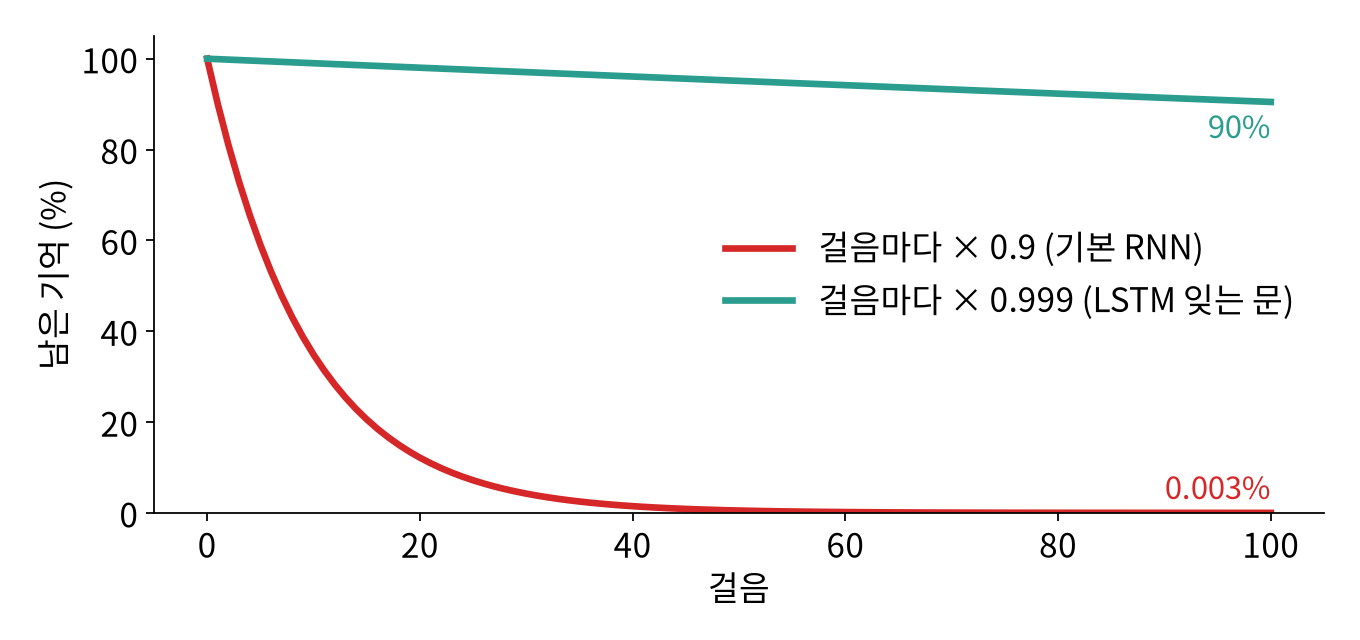
\includegraphics[width=0.6\linewidth]{ls_decay.png}\par\vskip0.2em
{\large 기본 RNN 처럼 걸음마다 기억에 0.9 를 곱하면 \quad $0.9^{100} \approx \kq{0.003\%}$ \quad 사실상 0}
\vfill
\note{지난 시간에 기본 RNN은 걸음마다 기억에 어떤 수를 곱하기 때문에 오래된 기억이 흐려진다고 했습니다. 예를 들어 걸음마다 0.9를 곱하면 100걸음 뒤에는 0.003퍼센트, 사실상 0입니다. 학습할 때도 100단어 전의 단어로 기울기가 전달되지 않아 오래전 일을 배우지 못합니다. 초록 선처럼 0.999를 곱하면 100걸음 뒤에도 90퍼센트가 남습니다. 오늘 배울 LSTM은 이 초록 선을 만드는 구조입니다.}
\end{frame}

% --- LSTM 아이디어
\begin{frame}{LSTM: 기억을 실어 나르는 컨베이어 벨트}
\markpage{cell}
\vfill
\centering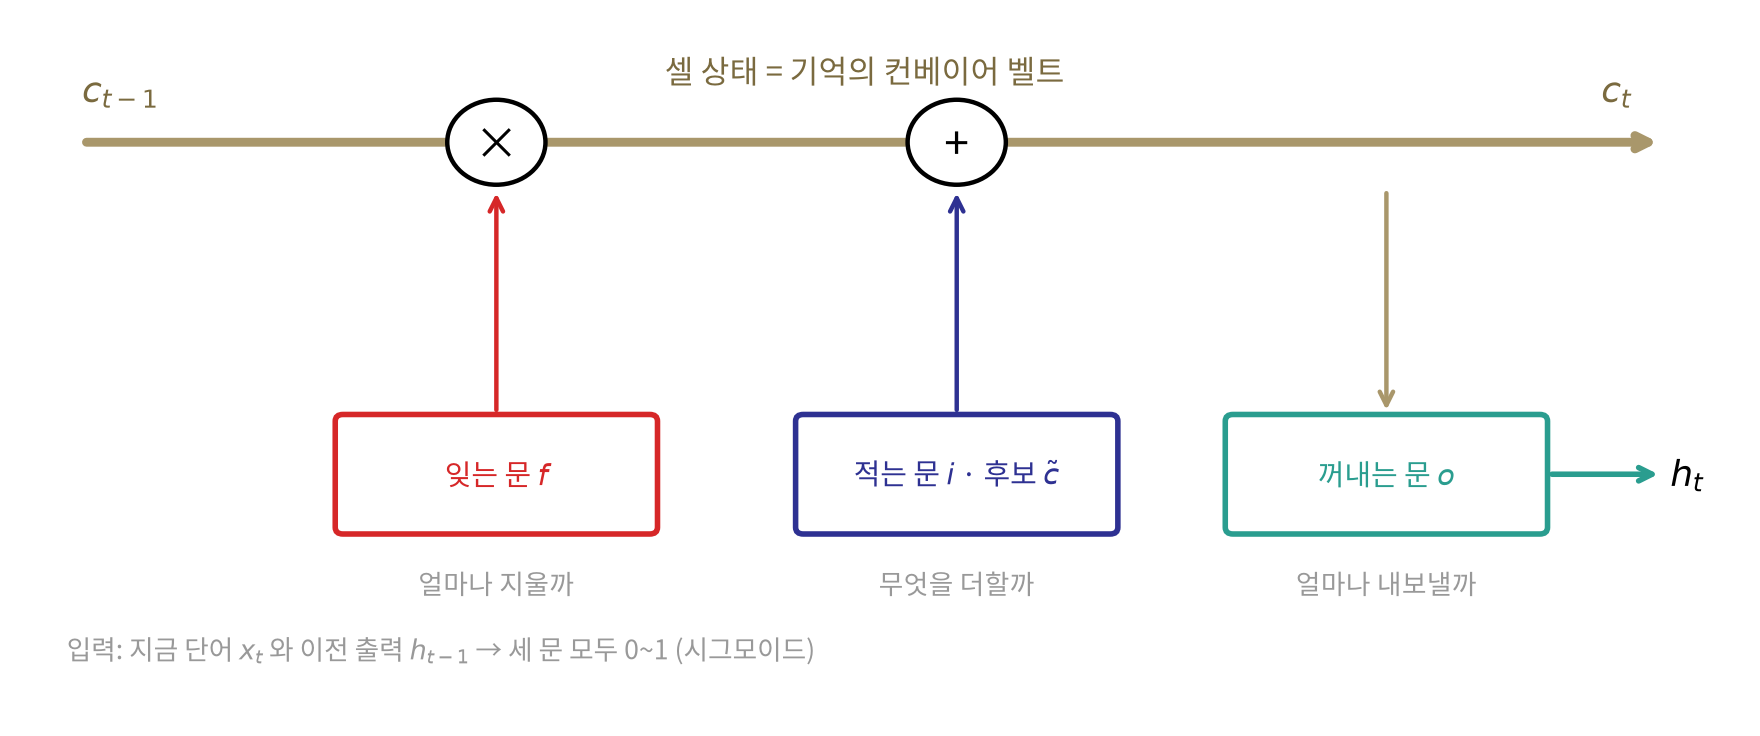
\includegraphics[width=0.8\linewidth]{ls_cell.png}\par\vskip0.2em
{\large 셀 상태 $c_t$ 는 \kb{더하기}로 이어진다 \quad 세 개의 \textbf{문 (gate)} 이 지우기 · 적기 · 꺼내기를 조절}\\[0.2em]
{\small Hochreiter \& Schmidhuber (1997) \quad 잊는 문은 Gers, Schmidhuber, Cummins (2000) 가 추가}
\vfill
\note{LSTM, 장단기 메모리는 1997년 호흐라이터와 슈미트후버가 발표했습니다. 핵심은 위쪽의 노란 선, 셀 상태라는 기억의 컨베이어 벨트입니다. 기본 RNN의 메모는 걸음마다 행렬을 곱하고 tanh를 씌우며 통째로 다시 쓰지만, 셀 상태는 거의 그대로 흘러가면서 필요한 만큼만 지우고 더합니다. 이걸 세 개의 문이 조절합니다. 잊는 문은 기억을 얼마나 지울지, 적는 문은 무엇을 더할지, 꺼내는 문은 기억 중 얼마를 출력으로 내보낼지 정합니다. 잊는 문은 2000년에 추가되어 지금의 LSTM이 되었습니다.}
\end{frame}

% --- 식
\begin{frame}{식으로}
\markpage{formula}
\vfill
\centering
{\large\[ \textcolor{ksared}{\mathbf{f}_t} = \sigma(W_f[\mathbf{h}_{t-1}, \mathbf{x}_t]) \qquad \textcolor{ksablue}{\mathbf{i}_t} = \sigma(W_i[\mathbf{h}_{t-1}, \mathbf{x}_t]) \]
\[ \mathbf{o}_t = \sigma(W_o[\mathbf{h}_{t-1}, \mathbf{x}_t]) \qquad \tilde{\mathbf{c}}_t = \tanh(W_c[\mathbf{h}_{t-1}, \mathbf{x}_t]) \]}\vskip0.2em
{\LARGE\[ \mathbf{c}_t = \textcolor{ksared}{\mathbf{f}_t} \odot \mathbf{c}_{t-1} + \textcolor{ksablue}{\mathbf{i}_t} \odot \tilde{\mathbf{c}}_t \qquad \mathbf{h}_t = \mathbf{o}_t \odot \tanh(\mathbf{c}_t) \]}\vskip0.2em
\renewcommand{\arraystretch}{1.2}
{\normalsize\begin{tabular}{ll}
$\sigma$: 0 $\sim$ 1 & 문은 ``얼마나 열지''를 칸마다 정한다 (0 = 닫힘, 1 = 활짝)\\
$\odot$ & 칸별 곱 \quad 편향은 생략해서 썼다
\end{tabular}}
\vfill
\note{식으로 쓰면 이렇습니다. 세 문 f, i, o와 후보 c 틸드는 모두 이전 출력 h와 지금 입력 x를 이어 붙여 각자의 가중치를 곱해 만듭니다. 문은 시그모이드라 0에서 1 사이, 얼마나 열지를 칸마다 정합니다. 후보는 tanh로 새로 적을 내용입니다. 새 셀 상태는 이전 셀 상태에 잊는 문을 곱한 것과, 후보에 적는 문을 곱한 것을 더한 것입니다. 출력 h는 셀 상태에 tanh를 씌우고 꺼내는 문을 곱한 것입니다. 가중치가 네 묶음이라 같은 크기의 RNN보다 가중치가 4배입니다.}
\end{frame}

% --- 손 계산
\begin{frame}{손으로 한 번 (기억 한 칸)}
\vfill
\centering
{\large 이전 기억 $c_{t-1} = 2$ \qquad 후보 $\tilde{c} = 0.8$\\[0.2em] 잊는 문 $f = 0.9$ \quad 적는 문 $i = 0.5$ \quad 꺼내는 문 $o = 0.7$}\vskip0.4em
{\LARGE\[ c_t = \underbrace{0.9 \times 2}_{\text{keep 90\%}} + \underbrace{0.5 \times 0.8}_{\text{write}} = 1.8 + 0.4 = \kb{2.2} \]}
{\LARGE\[ h_t = 0.7 \times \tanh(2.2) = 0.7 \times 0.976 = \kb{0.68} \]}\vskip0.2em
{\large 기억의 90\% 를 지키고, 새 내용을 절반만 더하고, 70\% 만 꺼내 보였다}
\vfill
\note{기억이 한 칸인 경우로 직접 계산해 봅니다. 이전 기억이 2, 잊는 문이 0.9, 적는 문이 0.5, 후보가 0.8, 꺼내는 문이 0.7입니다. 새 기억은 0.9 곱하기 2, 1.8에 0.5 곱하기 0.8, 0.4를 더해 2.2입니다. 기억의 90퍼센트를 지키고 새 내용을 절반만 더한 겁니다. 출력은 tanh 2.2, 0.976에 0.7을 곱해 0.68입니다. 기억 전체가 아니라 70퍼센트만 꺼내 다음 층과 다음 칸에 보여 준 겁니다.}
\end{frame}

% --- 왜 오래
\begin{frame}{왜 오래 기억할 수 있나}
\vfill
\centering
{\LARGE\[ \frac{\partial c_t}{\partial c_{t-1}} = f_t \qquad \text{(기본 RNN: } \tfrac{\partial h_t}{\partial h_{t-1}} = W_h \cdot \tanh'(\cdot)\text{)} \]}\vskip0.4em
{\large 셀 상태 경로에는 행렬도 tanh 도 없다 \quad 걸음마다 잊는 문 $f$ \textbf{하나만} 곱해진다}\\[0.6em]
{\large 기억해야 할 때 $f \approx 1$ 로 학습하면 \quad $0.999^{100} \approx \kb{90\%}$ \quad 기울기도 그대로 전달}\\[0.4em]
{\small 논문: 1,000걸음 넘게 떨어진 정보도 배울 수 있음을 보였다 \quad ResNet 의 지름길 (10주차) 과 같은 생각}
\vfill
\note{왜 오래 기억할 수 있을까요? 셀 상태를 이전 셀 상태로 미분하면 잊는 문 f 하나만 남습니다. 기본 RNN은 걸음마다 W_h 행렬과 tanh의 기울기를 곱해야 했는데, 셀 상태의 더하기 경로에는 행렬도 tanh도 없습니다. 그래서 기억해야 할 정보가 있을 때 잊는 문을 1에 가깝게 학습하면, 0.999의 100제곱처럼 기억과 기울기가 거의 그대로 전달됩니다. 원 논문은 1000걸음 넘게 떨어진 정보도 배울 수 있음을 보였습니다. 지난주 ResNet의 지름길이 깊이 방향의 더하기였다면, LSTM의 셀 상태는 시간 방향의 더하기입니다.}
\end{frame}

% --- 문의 뜻
\begin{frame}{문이 하는 일: 예}
\vfill
\centering
{\large ``The \textbf{cat}, which ate all the fish in the kitchen, \textbf{was} full''}\vskip0.8em
\renewcommand{\arraystretch}{1.5}
{\large\begin{tabular}{lll}
cat & \textcolor{ksablue}{적는 문} 열림 & 기억 칸 하나에 ``주어는 단수'' 를 적는다\\
which ate $\cdots$ kitchen & \textcolor{ksared}{잊는 문} $\approx 1$ & 그 칸을 지키며 지나간다\\
was & \textcolor{ksagolddk}{꺼내는 문} 열림 & ``단수'' 를 꺼내 was 를 고르게 한다\\
(문장 끝) & \textcolor{ksared}{잊는 문} $\approx 0$ & 다음 문장을 위해 지운다
\end{tabular}}\vskip0.6em
{\small 실제로 학습된 LSTM 에서 이렇게 해석되는 칸들이 발견된다 (예: 따옴표 안인지, 줄 길이) \quad Karpathy 외 (2015)}
\vfill
\note{문들이 하는 일을 예로 봅시다. The cat, which ate all the fish in the kitchen, was full이라는 문장에서, cat을 읽을 때 적는 문이 열려 기억 칸 하나에 주어가 단수라는 정보를 적습니다. which부터 kitchen까지는 잊는 문을 1에 가깝게 두고 그 칸을 지키며 지나갑니다. was를 고를 때 꺼내는 문이 열려 단수라는 정보를 꺼냅니다. 문장이 끝나면 잊는 문을 0 쪽으로 해 다음 문장을 위해 지웁니다. 물론 이건 해석이고 LSTM이 이렇게 하라고 배운 건 아니지만, 실제로 학습된 LSTM에서 따옴표 안에 있는지, 줄이 얼마나 길었는지를 기억하는 칸들이 발견되었습니다.}
\end{frame}

% --- 실험
\begin{frame}{실험: 셰익스피어 글자 모델, RNN vs LSTM}
\markpage{exp}
\vfill
\centering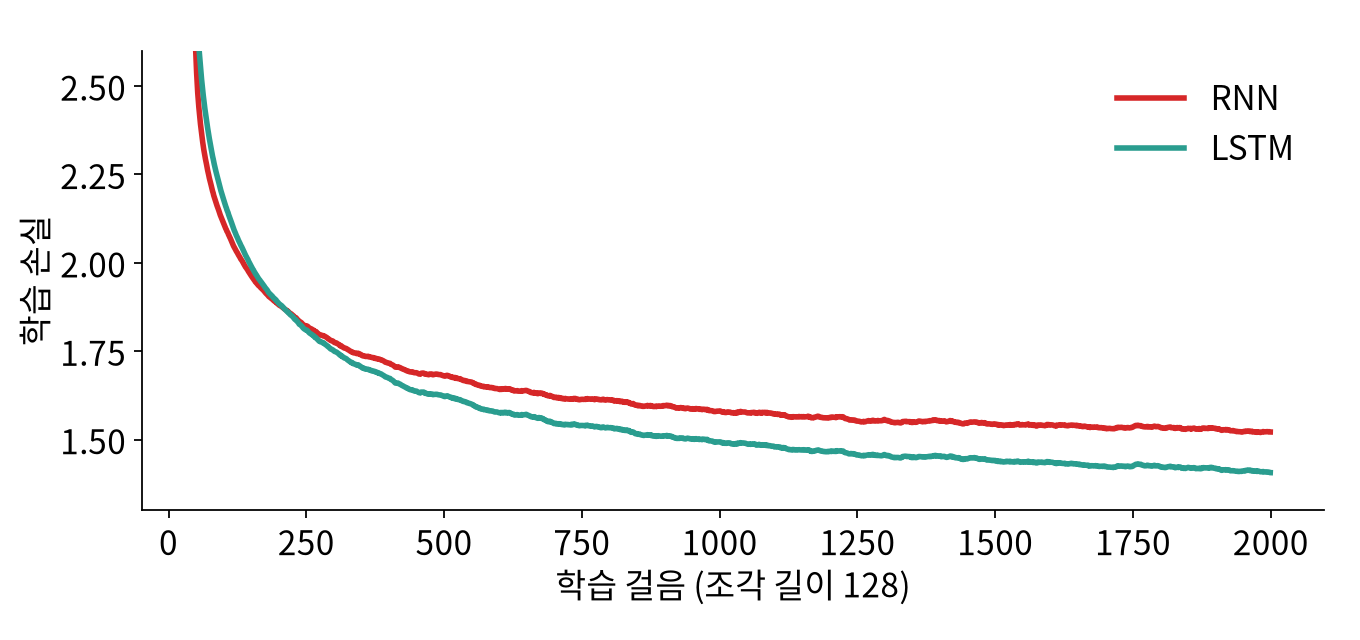
\includegraphics[width=0.56\linewidth]{ls_curve.png}\par\vskip0.2em
\renewcommand{\arraystretch}{1.2}
{\large\begin{tabular}{lcc}
검증 손실 (뒤 10\% 글) & 조각 64 & 조각 128\\\hline
RNN & 1.74 & 1.71\\
LSTM & \kb{1.64} & \kb{1.61}
\end{tabular}}
\vfill
\note{지난 시간의 셰익스피어 글자 모델을 RNN과 LSTM으로 똑같이 학습해 비교했습니다. 은닉 크기 128, 2000걸음, 같은 조건입니다. 학습 곡선에서 LSTM이 처음부터 더 빨리 내려갑니다. 학습에 쓰지 않은 뒤 10퍼센트 글로 잰 검증 손실은 조각 길이 64에서 1.74 대 1.64, 128에서 1.71 대 1.61로 LSTM이 낮습니다. 더 긴 앞부분을 활용할 수 있기 때문입니다.}
\end{frame}

% --- GRU
\begin{frame}{더 간단한 친척: GRU}
\vfill
\centering
{\large GRU (Gated Recurrent Unit, Cho 외 2014): 문 \textbf{두 개}, 셀 상태와 출력을 하나로}\vskip0.4em
{\LARGE\[ \mathbf{h}_t = (1 - \mathbf{z}_t) \odot \mathbf{h}_{t-1} + \mathbf{z}_t \odot \tilde{\mathbf{h}}_t \]}\vskip0.2em
{\large $\mathbf{z}$: 갱신 문 (잊기 + 적기를 한 번에) \quad 가중치가 LSTM 의 $\frac34$}\\[0.6em]
{\small 성능은 문제에 따라 LSTM 과 비슷 \quad PyTorch: \texttt{nn.LSTM}, \texttt{nn.GRU}}
\vfill
\note{LSTM의 간단한 친척인 GRU도 있습니다. 2014년 조경현 교수 팀이 제안했고, 문이 두 개입니다. 셀 상태와 출력을 하나로 합치고, 갱신 문 z 하나로 이전 기억을 얼마나 남기고 새 내용을 얼마나 넣을지 한 번에 정합니다. 1 빼기 z만큼 이전 것을, z만큼 새것을 섞는 식입니다. 가중치는 LSTM의 4분의 3이고, 성능은 문제에 따라 비슷합니다. PyTorch에서는 nn.LSTM과 nn.GRU로 바꿔 끼우기만 하면 됩니다.}
\end{frame}

% --- 역사
\begin{frame}{LSTM 이 활약한 곳}
\vfill
\centering
\renewcommand{\arraystretch}{1.5}
{\large\begin{tabular}{ll}
2014 & Seq2Seq 번역 (Sutskever 외): LSTM 4층, 영어 $\to$ 프랑스어\\
2015 $\sim$ 2016 & 음성 인식 · 구글 번역 (GNMT) 의 주력\\
2017 $\sim$ & 트랜스포머로 넘어간다: 모든 단어를 \textbf{한꺼번에} 본다
\end{tabular}}\vskip0.8em
{\large 그래도: 작은 시계열, 실시간 처리 (한 칸씩 들어오는 데이터) 에는 지금도 쓰인다}
\vfill
\note{LSTM은 2014년 Seq2Seq 번역에서 4층짜리 LSTM으로 영어를 프랑스어로 옮기며 큰 성공을 거뒀고, 2015년부터 음성 인식과 구글 번역의 주력이 되었습니다. 2017년 트랜스포머가 나오며 자리를 넘겨줬습니다. 트랜스포머는 단어를 하나씩이 아니라 한꺼번에 보기 때문에 멀리 떨어진 단어도 바로 연결하고, GPU로 병렬 계산도 쉽습니다. 그래도 작은 시계열이나 데이터가 한 칸씩 실시간으로 들어오는 경우에는 지금도 LSTM이 쓰입니다.}
\end{frame}

% --- 문제풀이
\begin{frame}{문제풀이}
\vfill
\begin{enumerate}
\item $c_{t-1} = 4$, $f = 0.5$, $i = 1$, $\tilde{c} = -1$ 이면 $c_t$ 는? $o = 1$ 이면 $h_t$ 는? ($\tanh 1 \approx 0.76$)\vskip0.8em
\item 잊는 문이 계속 0.99 면 100걸음 뒤 기억은 몇 \% 남나? ($0.99^{100} \approx 0.366$)\vskip0.8em
\item 입력 100칸, 은닉 128칸인 LSTM 층의 가중치 수는? (문 · 후보 4묶음, 각각 $[\mathbf{h}, \mathbf{x}]$ 에 곱하고 편향)\vskip0.8em
\item 문장이 끝날 때 잊는 문이 0 에 가까워지는 것이 왜 쓸모 있을까?
\end{enumerate}
\vfill
\note{1번 답. 0.5 곱하기 4, 2에 1 곱하기 마이너스 1을 더해 1이고, h는 tanh 1, 약 0.76입니다. 2번 답. 약 36.6퍼센트입니다. 3번 답. 묶음 하나가 128 곱하기 228에 편향 128, 29,312개이고, 4묶음이니 117,248개입니다. 4번 답. 이전 문장의 주어 같은 정보가 다음 문장에 섞여 들어가지 않게 기억을 비우는 겁니다.}
\end{frame}

% --- 실습
\begin{frame}{실습}
\vfill
\centering\begin{tabular}{rl}
\large 1 & LSTM 한 칸 직접 구현 $\to$ 손 계산 2.2 · 0.68, \texttt{nn.LSTMCell} 과 비교\\[0.5em]
\large 2 & 셰익스피어 글자 모델: \texttt{nn.RNN} vs \texttt{nn.LSTM} vs \texttt{nn.GRU}\\[0.5em]
\large 3 & 가중치 수 비교, 학습된 LSTM 으로 글 써 보기
\end{tabular}\vskip1em
Tiny Shakespeare (Karpathy, char-rnn) \\[0.4em]\href{https://colab.research.google.com/github/SuminHan/book-ml/blob/main/slides/v2/ml1/week11/lstm/lab/lstm.ipynb}{\textcolor{ksagolddk}{▶ Colab에서 실습 노트북 열기}}
\vfill
\note{실습은 세 부분입니다. 첫째, LSTM 한 칸을 numpy로 직접 구현해 손 계산을 재현하고 PyTorch LSTMCell과 비교합니다. 둘째, 셰익스피어 글자 모델을 RNN, LSTM, GRU로 학습해 손실을 비교합니다. 셋째, 세 모델의 가중치 수를 비교하고, 학습된 LSTM으로 글을 써 봅니다.}
\end{frame}

% --- 정리
\begin{frame}{정리}
\vfill
\centering\large\begin{tabular}{l}
기본 RNN: 걸음마다 곱해져 기억 · 기울기가 사라진다 ($0.9^{100} \approx 0.003\%$)\\[0.5em]
\textbf{LSTM}: 셀 상태 $c_t = f \odot c_{t-1} + i \odot \tilde{c}$ \quad \kb{더하기}로 이어지는 기억\\[0.5em]
세 문: 잊기 $f$ · 적기 $i$ · 꺼내기 $o$ (0 $\sim$ 1) \quad $f \approx 1$ 이면 오래 간다\\[0.5em]
셰익스피어 검증 손실 1.71 $\to$ 1.61 \quad GRU = 문 두 개 \quad 다음: Seq2Seq, 어텐션
\end{tabular}
\vfill
\note{정리합니다. 기본 RNN은 걸음마다 곱해져 기억과 기울기가 사라집니다. LSTM은 셀 상태라는 기억을 더하기로 이어서, 잊는 문만큼만 지우고 적는 문만큼 새로 더합니다. 세 문은 0에서 1 사이 값으로 지우기, 적기, 꺼내기를 칸마다 조절하고, 잊는 문이 1에 가까우면 기억이 오래 갑니다. 셰익스피어 실험에서 검증 손실이 1.71에서 1.61로 좋아졌고, 문이 두 개인 GRU도 있습니다. 다음 주에는 LSTM 두 개로 번역하는 Seq2Seq와, 그 한계를 푼 어텐션을 배웁니다.}
\end{frame}
\end{document}
